\chapter{Planteamiento}

Vamos a plantear de forma general una implementación y cómo aseguramos la calidad de la misma.

\section{Metodología}

Necesito una metodología que ponga al usuario en el centro y permita una retroalimentación rápida.\\
Aplicando técnicas de design thinking, se ha hecho un análisis de "Personas". **INCLUIR ANEXO**
\\
Lo ideal, es que estos conceptos que expongo más abajo tengan su representación en el sistema que utilicemos
para administrar estas tareas, en mi caso, GitHub. \\ \\
Por otra parte, es importante que \textbf{los commits referencien a estas tareas.} De esta forma, podemos
saber no solo quién ha escrito una línea de código sino también \textbf{por qué está ahí.} Es una forma de documentar el código.
\begin{figure}[H]
\centering	
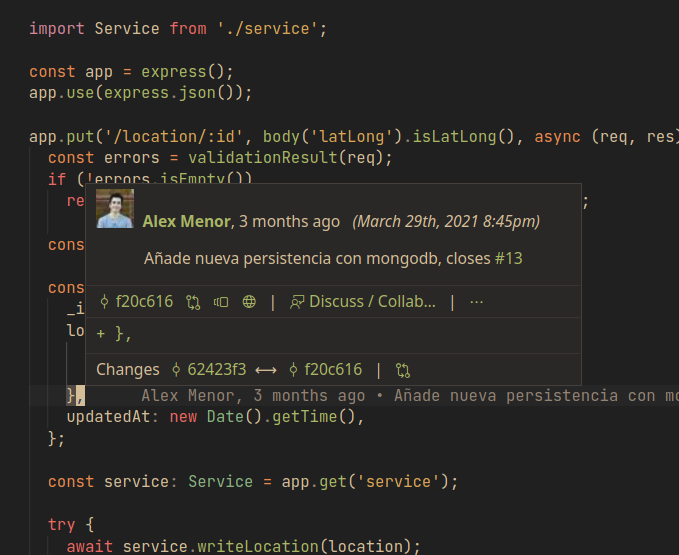
\includegraphics[scale=0.6]{git.png}
\end{figure}
\subsection{Iniciativas}
\textbf{Son grandes grupos de funcionalidad, independientes entre sí, que sirven para atacar el problema.}
Acorde a lo explicado en la sección \ref{sec:obj}, he propuesto las tres iniciativas y las he 
reflejado como proyectos dentro del repositorio de GitHub \cite{repo}.
\begin{figure}[H]
\centering	
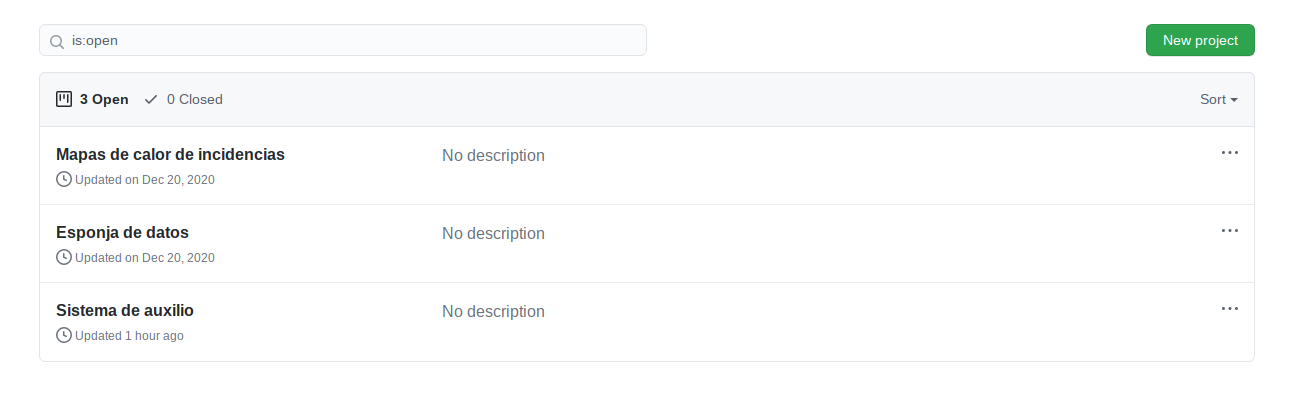
\includegraphics[scale=0.4]{iniciativas.png}
\end{figure}

\subsection{Épica}
Una iniciativa está formada por varias épicas. \textbf{Una épica por si sola no es una solución al problema}, pero todas las épicas de una iniciativa contribuyen a la solución.
Por ejemplo, para la iniciativa el sistema de auxilio, que es en la que se centra este trabajo, tenemos 
como épicas el frontend y el backend. Se reflejan en GitHub como milestones.
\begin{figure}[H]
	\centering
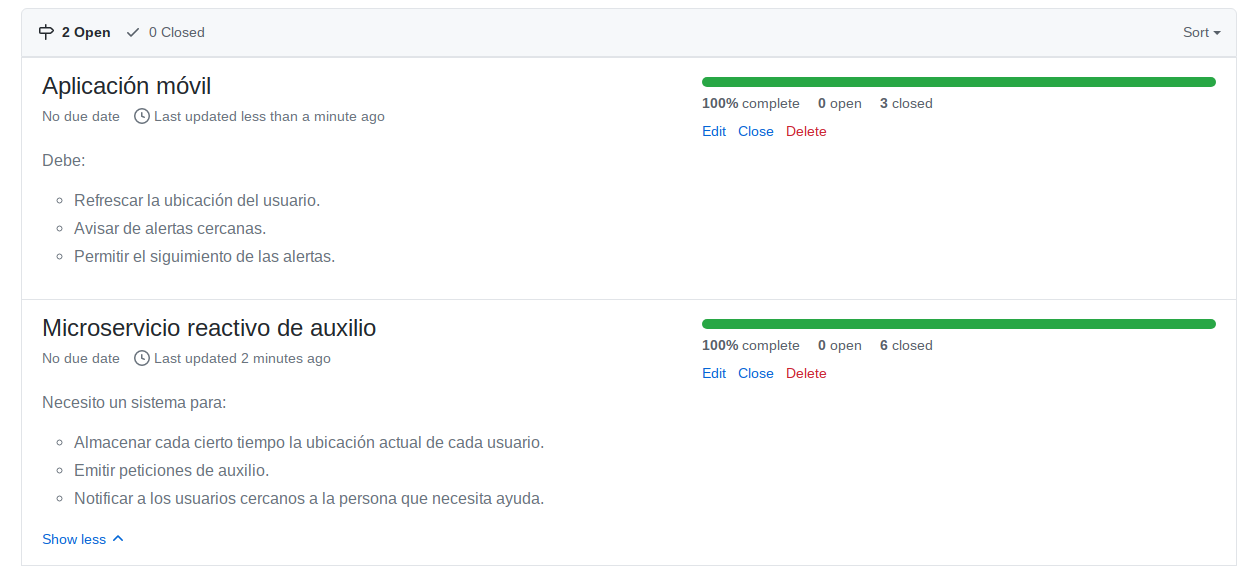
\includegraphics[scale=0.4]{milestones.png}
\end{figure}


\subsection{Historia de usuario}
Una épica a su vez está formada por varias historias de usuario que definen \textbf{una funcionalidad que el usuario espera en una solución}, de la forma:\\ \textit{Como [rol] quiero [funcionalidad] para [razón].}\\

A la hora de implementar una historia de usuario, esta se puede definir con requisitos más detallados.

\begin{figure}[H]
	\centering	
	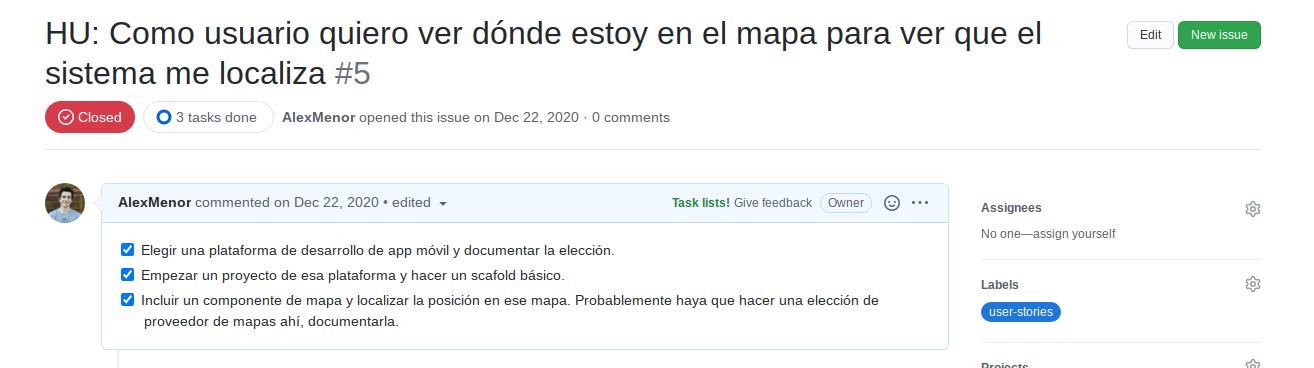
\includegraphics[scale=0.4]{hu.png}
	\end{figure}

\subsection{Issues}
Cuando no se obtiene el comportamiento esperado, podemos abrir un issue que se cerrará con un commit que lo solucione.

\begin{figure}[H]
	\centering	
	
\includegraphics[scale=0.4]{issue.png}
	\end{figure}

	También pueden ser issues tareas que faciliten el mantenimiento del código.

\begin{figure}[H]
	\centering	
	
\includegraphics[scale=0.4]{issue2.png}
	\end{figure}


\section{Quality assurance}

Para asegurar la calidad del proyecto necesitamos utilizar \textbf{integración continua con tests y análisis estático del código} por medio de linters (ver sección \ref{sec:tools}).


Cada vez que se hace un commit, se ejecutan todos estos procesos automáticamente.

La presencia de tests, de la que hablo con más detalle en la sección \ref{sec:tests}, nos permite, entre otras cosas, refactorizar con más 
tranquilidad. \\

Para cubrir la parte de integración continua he utilizado Github Actions,  configurando en formato \textit{yaml} todos los flujos.\\
La implementación continua de los tests y linters dependen del lenguaje y otros detalles de implementación, por tanto
son distintos para cada entorno.
\begin{figure}[H]
	\centering	
	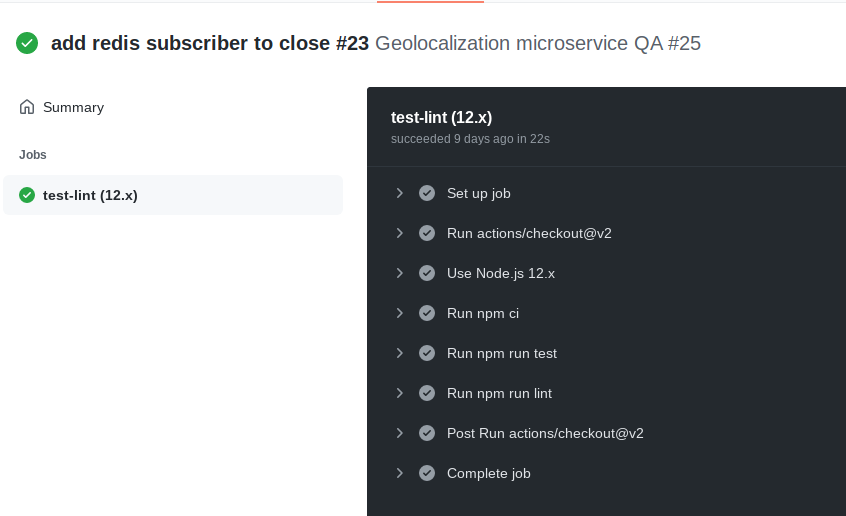
\includegraphics[scale=0.4]{ci.png}
	\end{figure}

\section{Planteamiento de implementación}

Tenemos dos partes bien diferenciadas.
\begin{itemize}
	\item  \textbf{La parte del cliente,} que se encargaría de actualizar con cierta frecuencia
la ubicación de cada usuario, recibir un aviso cuando haya alguien cercano que necesite ayuda y permitir realizar el seguimiento de una alerta.
\item Por otro lado, \textbf{la parte del servidor} recibe tanto las actualizaciones en cuanto a ubicación como 
los avisos de alerta. Se encarga por tanto de hacer los cálculos para saber a quién avisar y hacerlo. \\
Una vez la víctima y la persona que se presta a ayudar están conectadas, el servidor debe mantener
al cliente informado sobre la localización de la víctima y el estado de la alerta.
\end{itemize}


